% =====================================================================
\section{Prototipo: nodo \emph{edge} de alertas en tiempo real con conectividad intermitente}
\label{sec:prototipo}
% =====================================================================

La arquitectura de las secciones anteriores es deliberadamente amplia. Esta
sección delimita la parte que se implementa y se mide. El criterio de selección
fue elegir el problema tecnológico más crítico para que el resto de la
arquitectura funcione en una emergencia real: que la detección y las alertas no
dependan de un enlace que, en un desastre, es justamente lo primero que falla.

\subsection{Problema tecnológico y pregunta del prototipo}

En el diseño actual, las fuentes de campo (sensores IoT, drones) alimentan al
motor de interoperabilidad en la nube nacional. Si la detección de eventos
ocurre solo en la nube, cada alerta paga el viaje de ida y vuelta por la red
de área amplia (WAN) y, cuando el enlace cae, el municipio queda sin alertas y
los datos producidos durante la caída se pierden. El diagrama de despliegue
(figura~\ref{fig:c4-despliegue}) ya plantea un nodo \emph{edge} en el puesto de
mando unificado (PMU) con réplica local y agente de sincronización. El
prototipo construye ese nodo y lo somete a una caída controlada del enlace.

\begin{quote}
\itshape
¿Puede un nodo \emph{edge} municipal mantener la detección y la emisión de
alertas en tiempo real durante una caída del enlace con la nube, sin perder
lecturas, y converger con el nivel central al reconectarse sin generar
duplicados ni romper la trazabilidad?
\end{quote}

La pregunta se descompone en cinco hipótesis verificables:

\begin{enumerate}[leftmargin=*,label=\textbf{H\arabic*.}]
  \item La latencia de alerta en el \emph{edge} se mantiene por debajo de
        1\,s (p95), también durante la caída; la línea base solo nube paga la
        latencia de la WAN y pierde las alertas durante la caída.
  \item Ninguna lectura se pierde: tras la reconexión, la nube contiene
        exactamente el conjunto de lecturas producidas en campo.
  \item Los reenvíos causados por confirmaciones (ACK) perdidas no generan
        duplicados en la nube.
  \item El \emph{backlog} acumulado en el \emph{edge} se vacía en un tiempo
        acotado después de la reconexión.
  \item La bitácora de auditoría permanece íntegra y detecta cualquier
        alteración de un registro pasado.
\end{enumerate}

\subsection{Alcance: qué se construye y qué se simula}

La tabla~\ref{tab:alcance} responde la pregunta central de esta entrega. El
criterio es construir de verdad todo lo que está en la ruta crítica de la
hipótesis y simular lo que solo aporta datos o contexto. Los protocolos son
reales aunque el hardware sea simulado: los dispositivos publican por MQTT y la
sincronización viaja por HTTP a través de un enlace con latencia y cortes.

\begin{table}[htbp]
\centering
\caption{Delimitación del prototipo: componentes construidos, simulados y fuera de alcance.}
\label{tab:alcance}
\small
\begin{tabularx}{\textwidth}{@{}p{3.6cm}p{2.4cm}L@{}}
\toprule
\textbf{Elemento} & \textbf{Tratamiento} & \textbf{Detalle} \\
\midrule
\multicolumn{3}{@{}l}{\textit{Nodo edge del PMU (contenedores del diagrama de despliegue)}} \\
Broker MQTT & Construido & Mosquitto, QoS~1; recibe la telemetría de campo por la red local. \\
Ingesta y validación & Construido & Valida cada mensaje contra el contrato \texttt{Telemetry} y descarta reentregas por \texttt{event\_id}. \\
Detector de eventos & Construido & Umbrales por tipo de sensor y z-score móvil por dispositivo; enfriamiento de 10\,s para no repetir alertas del mismo episodio. \\
Almacén local con \emph{outbox} & Construido & SQLite en modo WAL; lectura y alerta se guardan en una sola transacción antes de cualquier envío. Materializa la réplica operacional local. \\
Agente de sincronización & Construido & Lotes de hasta 500 lecturas; marca como sincronizado solo con ACK; reintento con \emph{backoff} exponencial (0,5 a 8\,s). \\
Bitácora de auditoría & Construido & \emph{Append-only} encadenada con SHA-256: alertas, lotes sincronizados y cambios de estado del enlace. \\
COP local & Construido (mínimo) & Tablero web con alertas en vivo (\emph{Server-Sent Events}), estado del enlace y del \emph{backlog}. \\
\addlinespace
\multicolumn{3}{@{}l}{\textit{Nube nacional}} \\
API central & Construida (mínima) & Receptor idempotente de lotes (\texttt{POST /api/v1/sync}) y, para la línea base, ingesta directa con detección en la nube (\texttt{POST /api/v1/ingest}). \\
Base consolidada & Construida (mínima) & SQLite con \texttt{event\_id} como llave primaria. En producción sería la base operacional PostgreSQL/PostGIS. \\
\addlinespace
\multicolumn{3}{@{}l}{\textit{Entorno}} \\
Sensores y drones & Simulados & 50 dispositivos a 1\,Hz: 20 limnímetros, 15 pluviómetros, 10 acelerómetros y 5 drones con conteo de personas (el clasificador a bordo se simula). \\
Enlace WAN & Emulado & Proxy TCP propio: 200\,$\pm$\,80\,ms por sentido y corte controlado (cierra conexiones abiertas y rechaza nuevas). \\
Pérdida de ACK & Inyectada & La nube confirma la escritura pero responde 503 con probabilidad 0,1, para forzar reenvíos. \\
Respondientes locales & Simulados & Suscriptor MQTT que registra la hora de llegada de cada alerta. \\
\addlinespace
\multicolumn{3}{@{}l}{\textit{Fuera del prototipo}} \\
Optimización logística, IA sobre imágenes, GIS, interoperabilidad con SNIGRD/UNGRD, app de campo, autenticación & No se construyen & Siguen descritos en la arquitectura general; el prototipo no depende de ellos para responder la pregunta. \\
\bottomrule
\end{tabularx}
\end{table}

\subsection{Arquitectura del prototipo}

La figura~\ref{fig:prototipo} muestra los contenedores del prototipo con el
mismo nivel de detalle del nivel~2 de C4 (figura~\ref{fig:c4-contenedores}):
en azul lo construido, en gris discontinuo lo simulado o emulado. Los números indican el flujo
principal. El prototipo corresponde a tres contenedores del diagrama de
despliegue: COP local, agente de sincronización y réplica operacional local.
Agrega dos que el diseño general dejaba implícitos dentro del agente de
captura y del motor de interoperabilidad: el broker MQTT local y el detector de
eventos en el borde.

Los dos servicios construidos, el nodo \emph{edge} y la API de la nube, están
implementados en Java~21 con Spring Boot~3.5, como un proyecto Maven
multimódulo: un módulo compartido con los contratos y el detector, y un módulo
por servicio. El nodo \emph{edge} usa Eclipse Paho como cliente MQTT, SQLite
mediante Spring JDBC para el almacén local y \emph{Server-Sent Events} para el
COP; la nube expone su API con Spring MVC y la documenta con OpenAPI. Las
herramientas de prueba (simulador de dispositivos, emulador del enlace y
experimento) están en Python y solo hablan con los servicios a través de sus
contratos: MQTT, HTTP/JSON y el archivo SQLite del nodo \emph{edge}, que el
experimento lee para verificar la auditoría.

\begin{figure}[p]
  \centering
  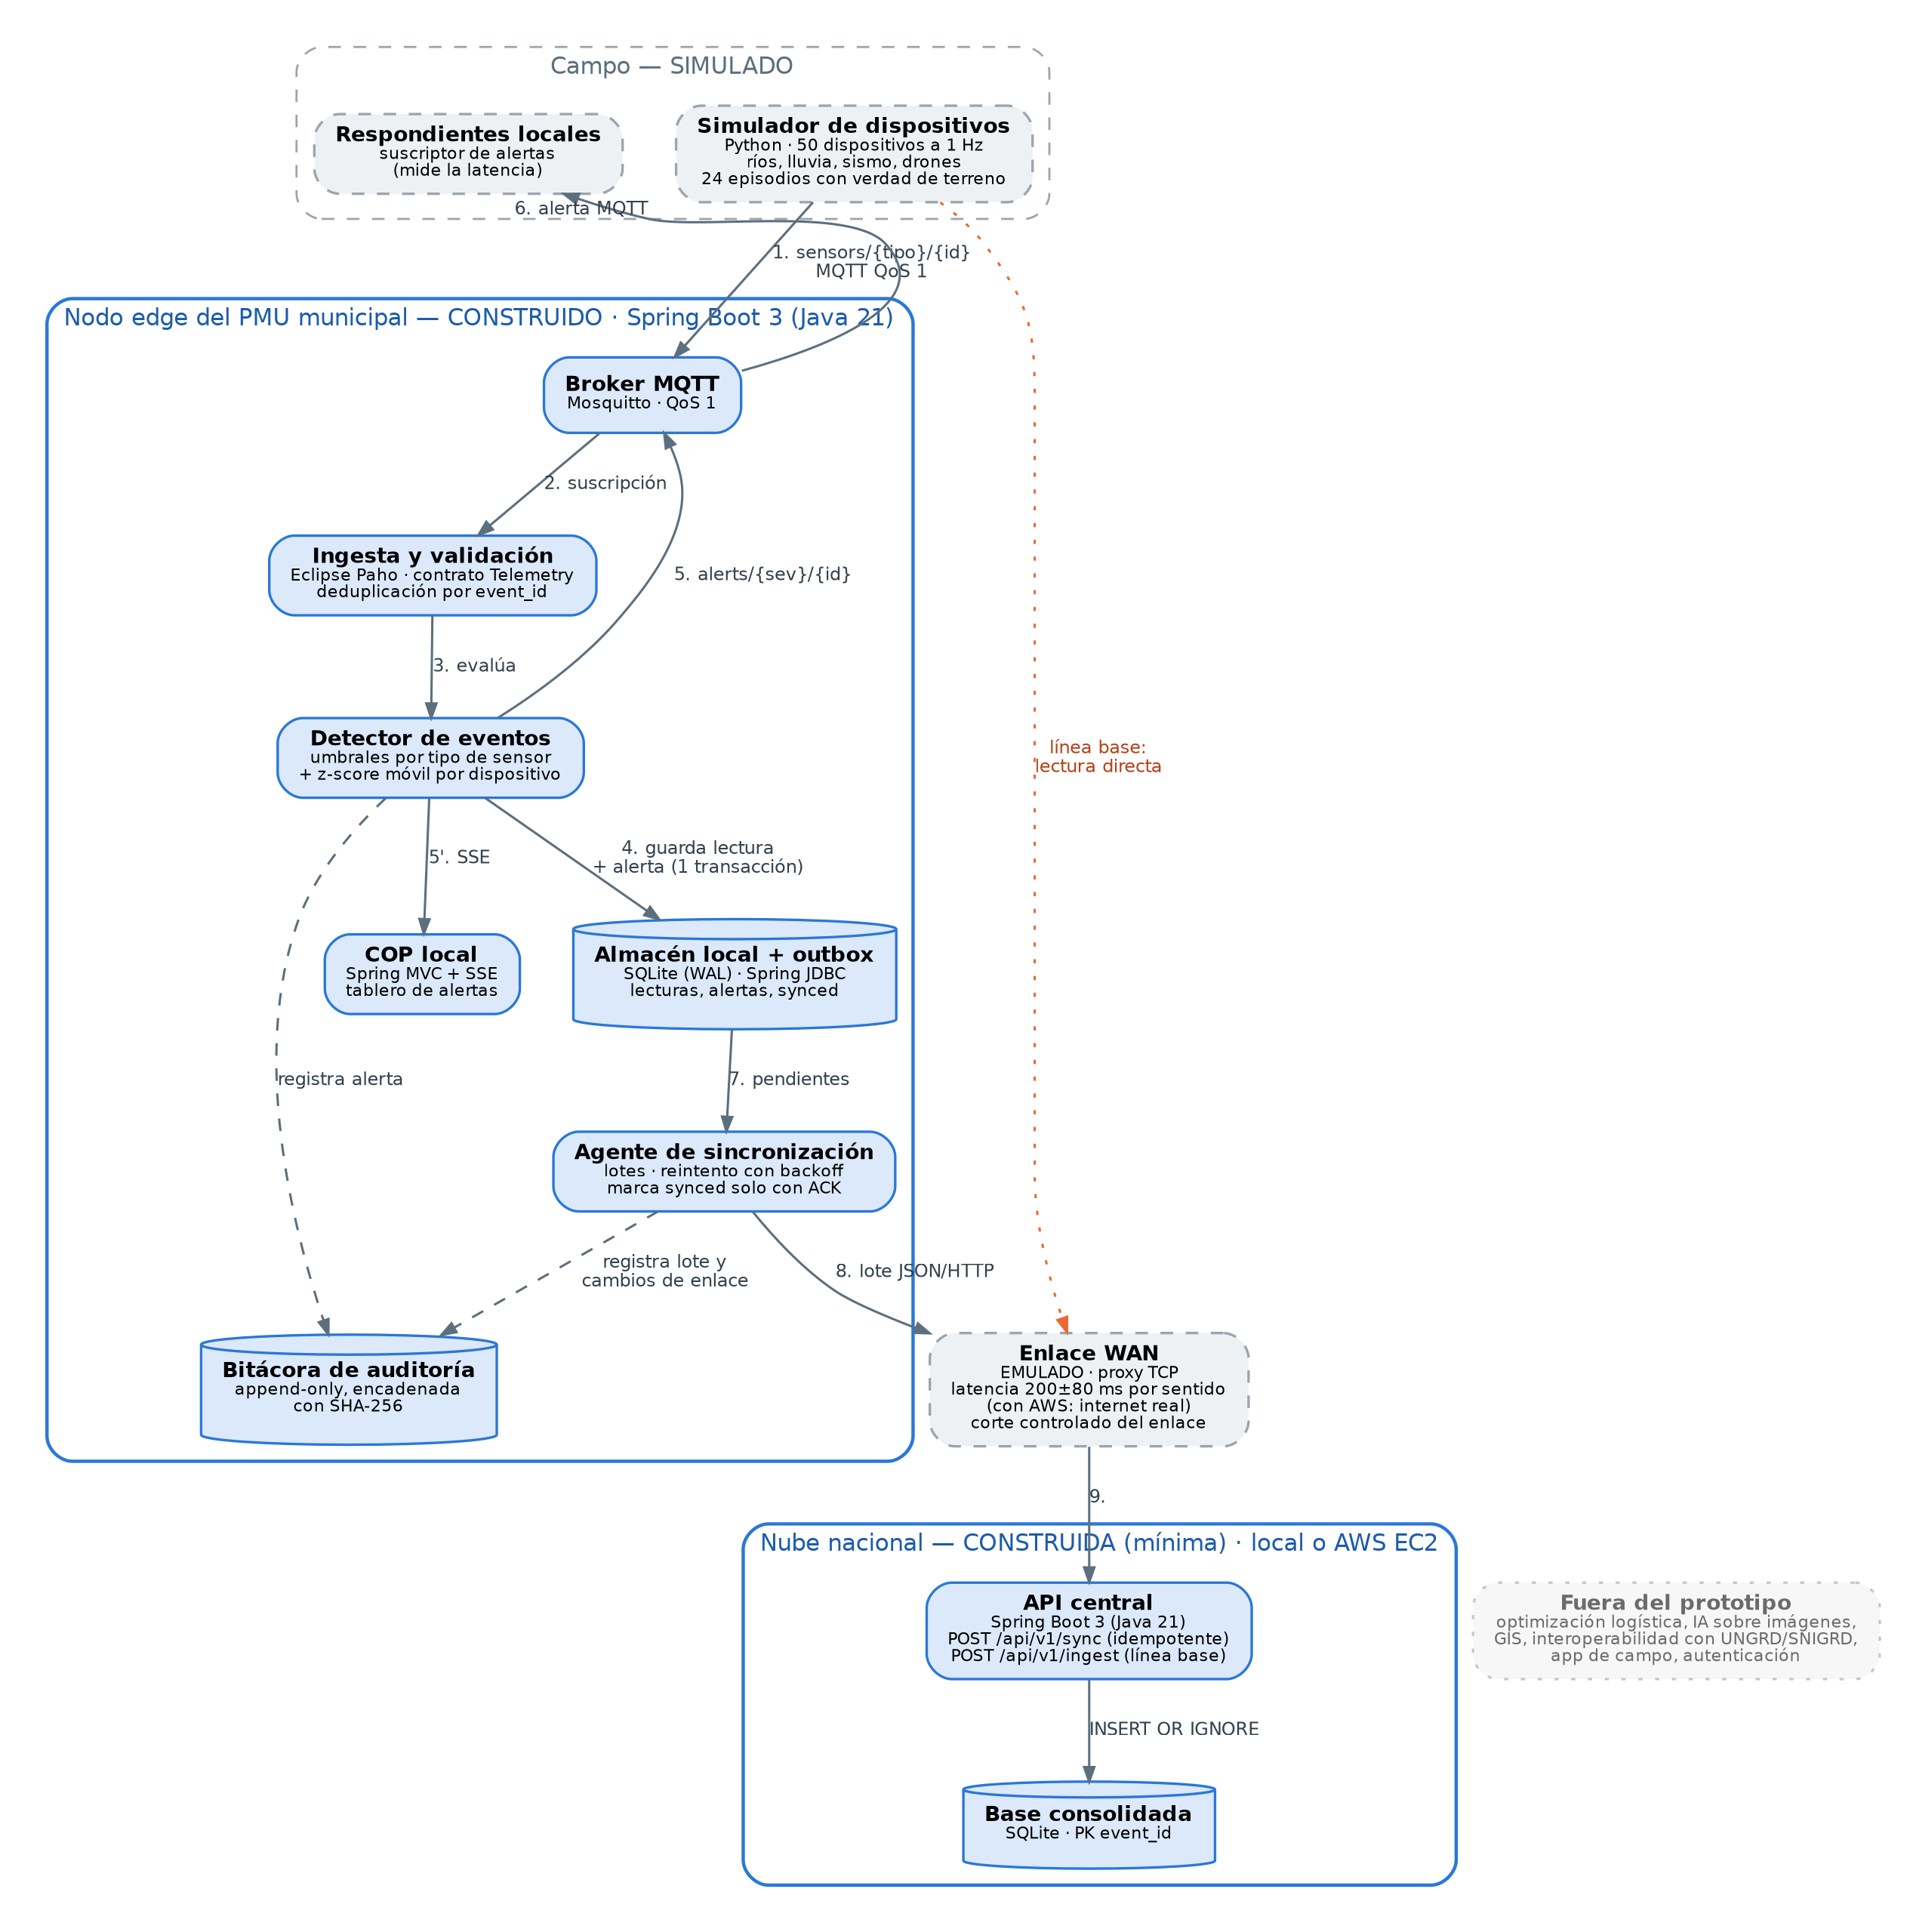
\includegraphics[width=\textwidth,height=0.86\textheight,keepaspectratio]{figuras/prototipo_contenedores.png}
  \caption{Contenedores del prototipo. Azul: construido. Gris discontinuo:
  simulado o emulado. Naranja punteado: ruta de la línea base solo nube.}
  \label{fig:prototipo}
\end{figure}

\subsection{Contratos}

Todos los mensajes que cruzan un límite de proceso tienen un contrato
explícito, versionado en el repositorio (\texttt{contracts/}) como JSON Schema
y OpenAPI, y validado en tiempo de ejecución. El \texttt{event\_id} (UUID
generado en el dispositivo) es la clave de idempotencia de extremo a extremo:
permite deduplicar en el \emph{edge} (reentregas QoS~1) y en la nube
(reenvíos de lotes).

\begin{table}[htbp]
\centering
\caption{Contratos implementados.}
\label{tab:contratos}
\small
\begin{tabularx}{\textwidth}{@{}p{3.1cm}p{3.6cm}L@{}}
\toprule
\textbf{Contrato} & \textbf{Canal} & \textbf{Campos clave y garantía} \\
\midrule
\texttt{Telemetry} & MQTT \texttt{sensors/\{tipo\}/\{id\}}, QoS~1 &
\texttt{event\_id}, \texttt{device\_id}, \texttt{sensor\_type}, \texttt{value},
\texttt{unit}, \texttt{lat}, \texttt{lon}, \texttt{seq}, \texttt{ts\_ms}.
Al menos una vez. \\
\addlinespace
\texttt{Alert} & MQTT \texttt{alerts/\{sev\}/\{id\}}, QoS~1, y SSE &
\texttt{alert\_id}, \texttt{event\_id}, \texttt{severity}, \texttt{rule},
\texttt{score}, \texttt{ts\_event\_ms}, \texttt{ts\_alert\_ms},
\texttt{source}. \\
\addlinespace
\texttt{SyncBatch} / \texttt{SyncAck} & HTTP \texttt{POST /api/v1/sync} &
Lote de lecturas y alertas; la respuesta informa aceptados y duplicados.
Idempotente: reenviar un lote no cambia el estado de la nube. \\
\addlinespace
\texttt{IngestResponse} & HTTP \texttt{POST /api/v1/ingest} &
Solo para la línea base: el dispositivo envía la lectura y recibe la alerta en
la respuesta. \\
\bottomrule
\end{tabularx}
\end{table}

\subsection{Datos}

No se usan datos reales de sensores. El simulador genera un escenario
reproducible (semilla fija) alrededor de coordenadas plausibles de un
municipio de Putumayo. Sobre el ruido normal de cada dispositivo se plantan 24
episodios anómalos de 6\,s, en dispositivos distintos y repartidos a lo largo
de la ejecución, de modo que 12 caen dentro de la ventana de caída: cinco
desbordamientos de río (sobre el umbral crítico), cinco crecidas súbitas que
no alcanzan el umbral y solo detecta el z-score, cinco lluvias intensas, cinco
movimientos sísmicos y cuatro detecciones de personas por dron. El simulador
registra la primera lectura anómala de cada episodio como verdad de terreno,
lo que permite medir de forma objetiva la latencia, la sensibilidad
(\emph{recall}) y la precisión de las alertas.

\subsection{Flujos}

\begin{enumerate}[leftmargin=*]
  \item \textbf{Operación normal.} Dispositivo $\rightarrow$ broker
        $\rightarrow$ ingesta $\rightarrow$ detector $\rightarrow$ almacén
        local (lectura y alerta en una transacción) $\rightarrow$ alerta por
        MQTT y SSE a los respondientes y al COP local. En paralelo, el agente
        de sincronización envía los pendientes a la nube cada 0,5\,s.
  \item \textbf{Caída del enlace.} El agente detecta el error, registra
        \texttt{link\_down} en la auditoría y entra en \emph{backoff}. La
        detección y las alertas continúan sin cambios porque no dependen de la
        nube; las lecturas se acumulan como pendientes en el almacén local.
  \item \textbf{Reconexión.} El siguiente reintento tiene éxito, se registra
        \texttt{link\_up} y el agente vacía el \emph{backlog} en lotes
        consecutivos sin espera.
  \item \textbf{ACK perdido.} La nube guarda el lote pero la confirmación no
        llega. El \emph{edge} no marca las filas y las reenvía; la nube las
        reconoce como duplicadas por llave primaria y no las vuelve a guardar.
  \item \textbf{Línea base solo nube.} Cada dispositivo envía su lectura a la
        nube por la WAN; la nube detecta y devuelve la alerta. Durante la caída
        los envíos fallan y no hay alerta.
\end{enumerate}

\subsection{Decisiones de diseño del prototipo}

\begin{table}[htbp]
\centering
\caption{Decisiones del prototipo, alternativa descartada y justificación.}
\label{tab:adr-prototipo}
\small
\begin{tabularx}{\textwidth}{@{}p{3.6cm}LL@{}}
\toprule
\textbf{Decisión} & \textbf{Alternativa descartada} & \textbf{Justificación} \\
\midrule
MQTT con QoS~1 entre campo y \emph{edge} & HTTP por lectura & Protocolo
estándar de IoT, liviano para enlaces de radio; QoS~1 asegura entrega a cambio
de posibles duplicados, que se resuelven por \texttt{event\_id}. \\
\addlinespace
Patrón \emph{outbox} en SQLite & Enviar directo a la nube y guardar después &
Si el envío falla, el dato ya está persistido; la caída solo hace crecer el
\emph{backlog}. \\
\addlinespace
Receptor idempotente en la nube & Garantizar entrega exactamente una vez en el
transporte & \emph{Exactly-once} en red no es alcanzable; \emph{al menos una
vez} más idempotencia da el mismo efecto observable con un mecanismo simple. \\
\addlinespace
Detección por reglas y z-score & Modelo de aprendizaje profundo en el borde &
Explicable, sin entrenamiento y con costo de cómputo despreciable; un modelo
entrenado es trabajo futuro y se integraría en el mismo punto. \\
\addlinespace
\emph{Backoff} exponencial con tope de 8\,s & Reintento constante e inmediato &
Evita saturar un enlace degradado; el costo es una demora de hasta 8\,s en
notar la reconexión (se mide en H4). \\
\addlinespace
Auditoría encadenada con \emph{hash} & Tabla de registro sin protección &
Cualquier alteración de un registro pasado rompe la cadena desde ese punto y
queda localizada. \\
\bottomrule
\end{tabularx}
\end{table}

\subsection{Diseño experimental}

Se ejecuta el mismo escenario de 120\,s (6\,000 lecturas) dos veces sobre la
misma infraestructura: una con el nodo \emph{edge} y otra con la línea base
solo nube. En ambas, el enlace WAN cae entre los segundos 40 y 80. En la
ejecución \emph{edge} se inyecta además la pérdida del 10\,\% de los ACK. La
latencia de alerta se mide como el tiempo entre la primera lectura anómala de
un episodio y la llegada de su primera alerta al lado de los respondientes
locales. Un episodio cuenta como detectado si al menos una de sus lecturas
genera alerta. Una alerta es verdadera si su lectura pertenece a algún
episodio. Al final se comparan los identificadores de lecturas producidas con
los almacenados en la nube.

Como prueba complementaria de capacidad, se ejecuta el \emph{edge} sin caída
con 500 dispositivos simulados a 10\,Hz (500 mensajes por segundo durante
40\,s). Para H5 se copia la base local, se altera una entrada intermedia de la
bitácora y se verifica la cadena.

El entorno de medición fue un único equipo Windows~11 con Docker Desktop:
nodo \emph{edge} y nube en Spring Boot~3.5 sobre Java~21, broker Mosquitto~2 y
herramientas de prueba en Python~3.13, todos en contenedores. La WAN emulada es
la única fuente de latencia de red.

\subsection{Resultados}

La tabla~\ref{tab:resultados} resume las métricas y las
figuras~\ref{fig:latencia} y~\ref{fig:timeline} muestran su comportamiento.

\begin{table}[htbp]
\centering
\caption{Resultados del experimento: mismo escenario, caída de 40\,s del enlace.}
\label{tab:resultados}
\small
\begin{tabularx}{\textwidth}{@{}Lrr@{}}
\toprule
\textbf{Métrica} & \textbf{Solo nube} & \textbf{Edge} \\
\midrule
Lecturas generadas & 6\,000 & 6\,000 \\
Lecturas perdidas & 2\,012 (33.5 \%) & 0 (0.0 \%) \\
Episodios detectados (recall) & 14/24 (0.58) & 24/24 (1.00) \\
Episodios detectados durante la caída & 2/12 & 12/12 \\
Precisión de las alertas & 1.00 & 1.00 \\
Latencia de alerta p50 (ms) & 448 & 2 \\
Latencia de alerta p95 (ms) & 2\,379 & 23 \\
Duplicados almacenados en la nube & 0 & 0 \\
Reenvíos rechazados por idempotencia & -- & 263 \\
Backlog máximo en edge (lecturas) & -- & 2\,448 \\
Vaciado del backlog tras reconectar (s) & -- & 9.8 \\
\bottomrule
\end{tabularx}

\end{table}

\begin{figure}[htbp]
  \centering
  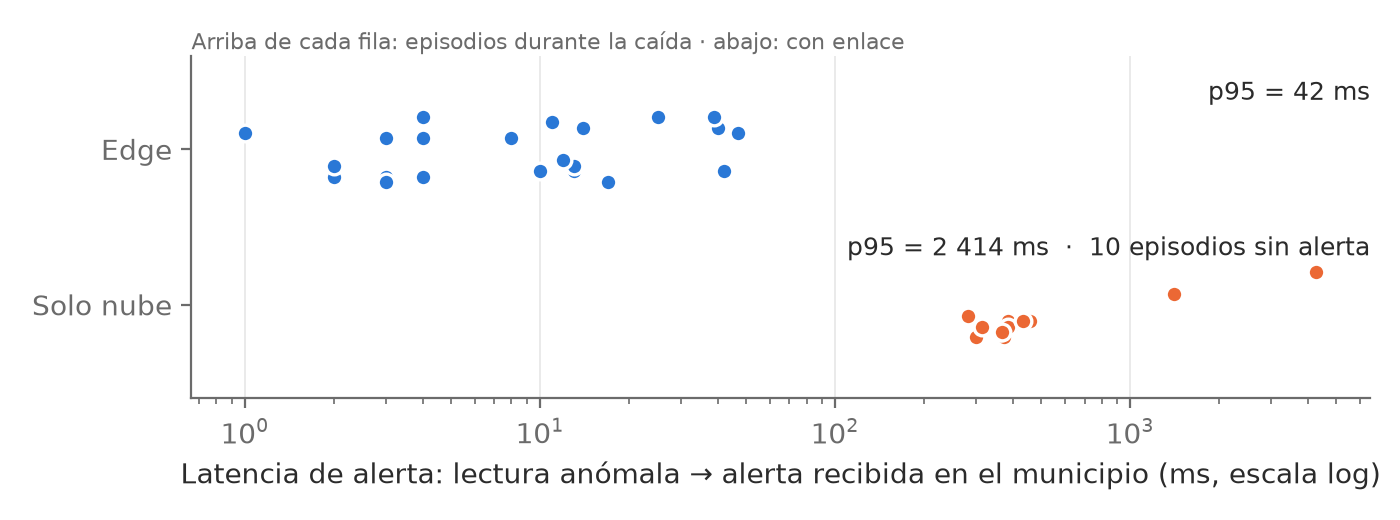
\includegraphics[width=\textwidth]{figuras/fig_latencia_alertas.png}
  \caption{Latencia de alerta por episodio detectado (escala logarítmica). Los
  diez episodios que la línea base no detecta ocurrieron durante la caída.}
  \label{fig:latencia}
\end{figure}

\begin{figure}[htbp]
  \centering
  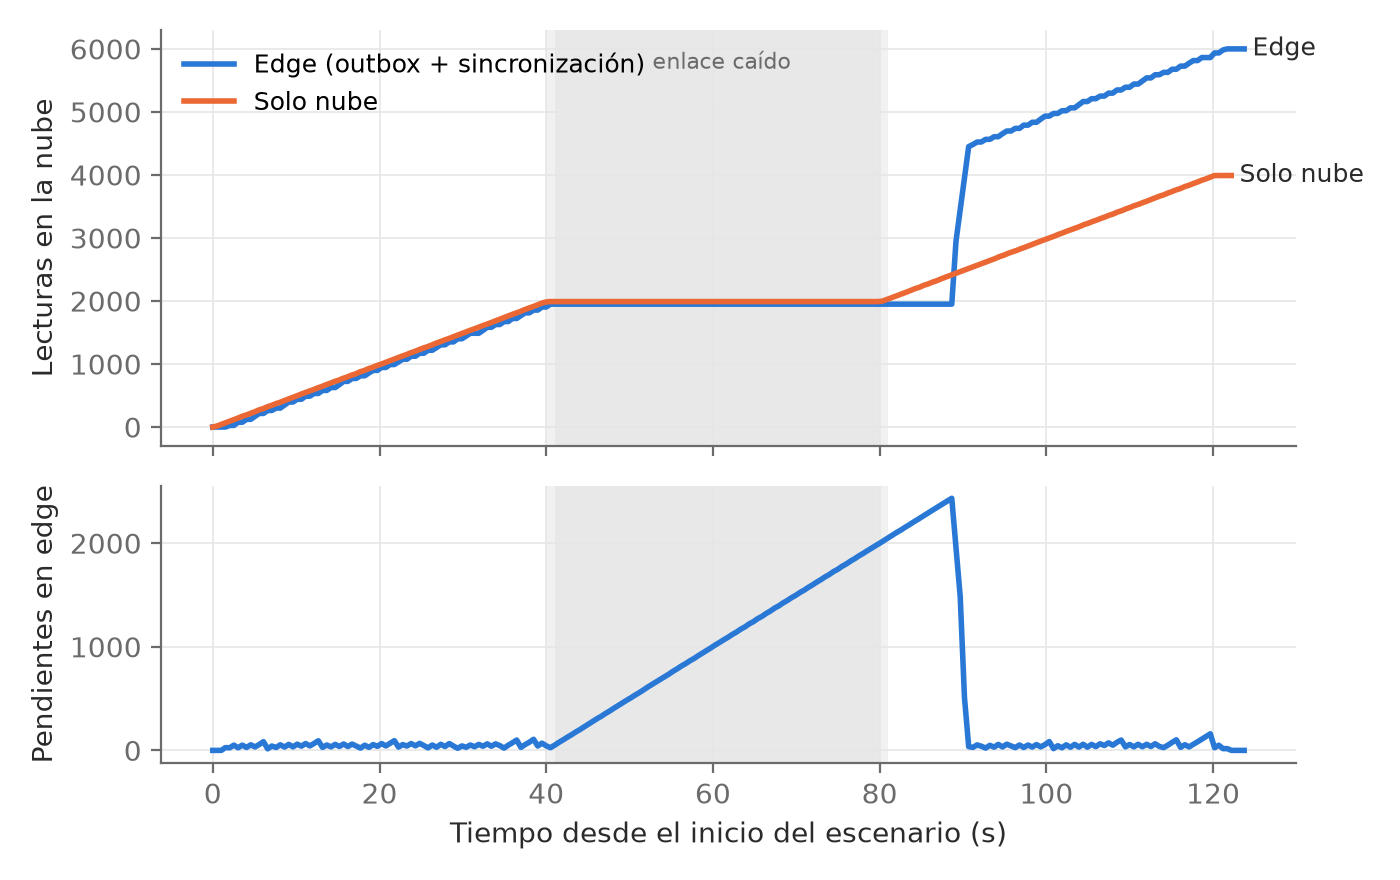
\includegraphics[width=\textwidth]{figuras/fig_linea_tiempo.png}
  \caption{Arriba: lecturas almacenadas en la nube en cada ejecución. Abajo:
  lecturas pendientes de sincronizar en el nodo \emph{edge}. La franja gris es
  la caída del enlace.}
  \label{fig:timeline}
\end{figure}

\textbf{H1 (latencia y continuidad).} Se cumple. El \emph{edge} entregó las
alertas con una mediana de 10,5\,ms y un p95 de 42\,ms (máximo 47\,ms), sin
diferencia apreciable durante la caída. La línea base tuvo una mediana de
380\,ms y un p95 de 2\,414\,ms. Con el enlace disponible su p95 fue 445\,ms,
casi todo el viaje de ida y vuelta por la WAN. Durante la caída solo generó
alerta para 2 de 12 episodios, y únicamente porque esos episodios seguían
activos cuando volvió el enlace, con 1,4 y 4,3\,s de retraso. El \emph{edge}
detectó los 24 episodios (19 por umbral y 5 crecidas súbitas por z-score), sin
falsas alarmas en ninguna de las dos ejecuciones.

\textbf{H2 (sin pérdida).} Se cumple. La nube terminó con las 6\,000 lecturas
producidas en la ejecución \emph{edge}. La línea base perdió 2\,009 (33,5\,\%):
todo lo producido durante los 40\,s de caída.

\textbf{H3 (sin duplicados).} Se cumple. Las diez pérdidas de ACK inyectadas
provocaron el reenvío de 502 lecturas que la nube ya tenía; todas fueron
reconocidas como duplicadas y no se almacenó ninguna dos veces.

\textbf{H4 (convergencia).} Se cumple, con un hallazgo de diseño. El
\emph{backlog} llegó a 2\,433 lecturas y volvió a su nivel normal (p95 de 88
pendientes con enlace) 9,7\,s después de la reconexión. De ese tiempo, 8,1\,s
transcurrieron antes del primer reintento exitoso, porque el agente estaba en
la espera máxima del \emph{backoff}; el vaciado como tal tomó cerca de 1,6\,s.
El tope del \emph{backoff} es, por tanto, el parámetro que domina la
convergencia. Un sondeo liviano del enlace mientras se espera reduciría ese
tiempo sin volver a saturar la red.

\textbf{H5 (auditoría).} Se cumple. La cadena de 116 entradas se verificó
íntegra. Al alterar la entrada 58 en una copia de la base, la verificación la
señaló como la primera entrada inválida. La cadena la escribe el nodo
\emph{edge} en Java y la verifica un programa independiente en Python, lo que
confirma además que el formato es reproducible fuera del sistema que lo genera.

\textbf{Capacidad.} Con 500 mensajes por segundo el \emph{edge} procesó las
20\,000 lecturas sin acumular cola, con un tiempo de procesamiento por mensaje
de 0,26\,ms (p95) y 0,52\,ms (p99), una latencia de alerta p95 de 6,4\,ms y
todos los episodios detectados.

\subsection{Validación con la nube desplegada en AWS}
\label{sec:prototipo-aws}

Para comprobar que los resultados no dependen de la WAN emulada, la API de la
nube se desplegó en una instancia EC2 de AWS (Amazon Linux 2023, t3.medium,
región us-east-1, en el AWS Academy Learner Lab). El nodo \emph{edge}, el
broker, el emulador del enlace y el simulador siguieron en el portátil, que
hace las veces de puesto de mando municipal. Así, el enlace \emph{edge}--nube
atraviesa internet de verdad: el emulador queda con latencia y jitter en cero y
solo se usa para cortar el enlace de forma controlada. El \emph{security group}
de la instancia admite conexiones únicamente desde la IP pública del puesto de
mando, y un script de PowerShell enciende la instancia, actualiza esa regla y
levanta el entorno local en cada sesión, porque el laboratorio apaga la
instancia y cambia su IP al terminar.

La tabla~\ref{tab:resultados-aws} compara el mismo experimento con la WAN
emulada y con la nube en AWS.

\begin{table}[htbp]
\centering
\caption{Mismo experimento con WAN emulada (200\,$\pm$\,80\,ms por sentido) y con
la nube desplegada en AWS (internet real hasta us-east-1).}
\label{tab:resultados-aws}
\small
\begin{tabular}{@{}lrrrr@{}}
\toprule
& \multicolumn{2}{c}{\textbf{Solo nube}} & \multicolumn{2}{c}{\textbf{Edge}} \\
\cmidrule(lr){2-3}\cmidrule(l){4-5}
\textbf{Métrica} & \textbf{Emulada} & \textbf{AWS} & \textbf{Emulada} & \textbf{AWS} \\
\midrule
Lecturas perdidas (de 6\,000) & 2\,009 & 1\,999 & 0 & 0 \\
Episodios detectados & 14/24 & 14/24 & 24/24 & 24/24 \\
Detectados durante la caída & 2/12 & 2/12 & 12/12 & 12/12 \\
Latencia de alerta p50 (ms) & 380 & 129 & 10,5 & 8 \\
Latencia de alerta p95 (ms) & 2\,414 & 2\,615 & 42 & 36 \\
Duplicados almacenados en la nube & 0 & 0 & 0 & 0 \\
Vaciado del \emph{backlog} (s) & -- & -- & 9,7 & 2,4 \\
\bottomrule
\end{tabular}
\end{table}

Las cinco hipótesis se mantienen con la nube real. La latencia de la línea base
es menor que con la WAN emulada (mediana de 129\,ms frente a 380\,ms), porque el
viaje de ida y vuelta real hasta us-east-1 resultó más corto que los 400\,ms
emulados; aun así es más de un orden de magnitud mayor que la del \emph{edge},
y la caída le sigue costando un tercio de las lecturas y 10 de los 12
episodios. El vaciado más rápido del \emph{backlog} no es una mejora del
sistema: en esa ejecución el primer reintento exitoso llegó 1,7\,s después de
la reconexión, frente a 8,1\,s, según en qué punto de la espera del
\emph{backoff} estaba el agente. El hallazgo de H4 sigue vigente.

\subsection{Limitaciones y amenazas a la validez}

\begin{itemize}[leftmargin=*]
  \item Las mediciones principales corrieron en un solo equipo; la
        validación de la sección~\ref{sec:prototipo-aws} llevó la nube a AWS,
        pero el nodo \emph{edge}, el broker y los dispositivos simulados
        siguieron en el mismo equipo. La red local entre campo y \emph{edge}
        no tiene latencia; en una red de radio real se sumarían decenas a
        cientos de milisegundos a la latencia del \emph{edge}, que seguiría
        lejos de la línea base y, sobre todo, no dependería de la WAN.
  \item Los datos son sintéticos y los episodios son claros. Las cifras de
        precisión y \emph{recall} prueban que el flujo funciona, no la calidad
        del detector frente a señales reales; para eso hacen falta series
        históricas de estaciones del IDEAM o de redes de monitoreo locales.
  \item La línea base no almacena lecturas en el dispositivo durante la caída.
        Si lo hiciera, evitaría la pérdida de datos pero sus alertas
        llegarían, como mínimo, con el retraso de la caída completa.
  \item SQLite en modo WAL con \texttt{synchronous=NORMAL} resiste la caída del
        proceso pero no un corte de energía del equipo; en producción el nodo
        usaría PostgreSQL con escritura sincrónica.
  \item Solo se modeló un nodo \emph{edge}. Varios municipios sincronizando a
        la vez y la resolución de conflictos sobre datos editados en ambos
        lados quedan como trabajo siguiente.
\end{itemize}

\subsection{Reproducibilidad}

El código fuente acompaña este documento: es un proyecto Maven multimódulo
cuya raíz contiene el \texttt{pom.xml}, el \emph{wrapper} \texttt{mvnw}, los
módulos \texttt{shared/}, \texttt{edge-node/} y \texttt{cloud-api/}, y las
herramientas de prueba en Python. \texttt{mvnw verify} ejecuta las pruebas
unitarias (JUnit). \texttt{docker compose up -{}-build} levanta el broker, el
nodo \emph{edge}, el enlace emulado y la nube. \texttt{docker compose -{}-profile
experiment run -{}-rm experiment} repite el experimento completo y regenera la
tabla~\ref{tab:resultados} y las figuras~\ref{fig:latencia}
y~\ref{fig:timeline}. Sin Docker, \texttt{mvnw package} seguido de
\texttt{python scripts/run\_local\_stack.py} levanta los mismos servicios como
procesos locales. Con la nube en AWS, \texttt{scripts/aws-up.ps1} enciende la
instancia y levanta el resto con \texttt{docker-compose.aws.yml}; el
procedimiento está en \texttt{docs/aws/despliegue-aws.md}. El tablero del COP
local queda en \texttt{http://localhost:8080}.
